\section{Classes}



\subsection{Server tier class diagram}
TODOO sentence about this dia
\begin{center}
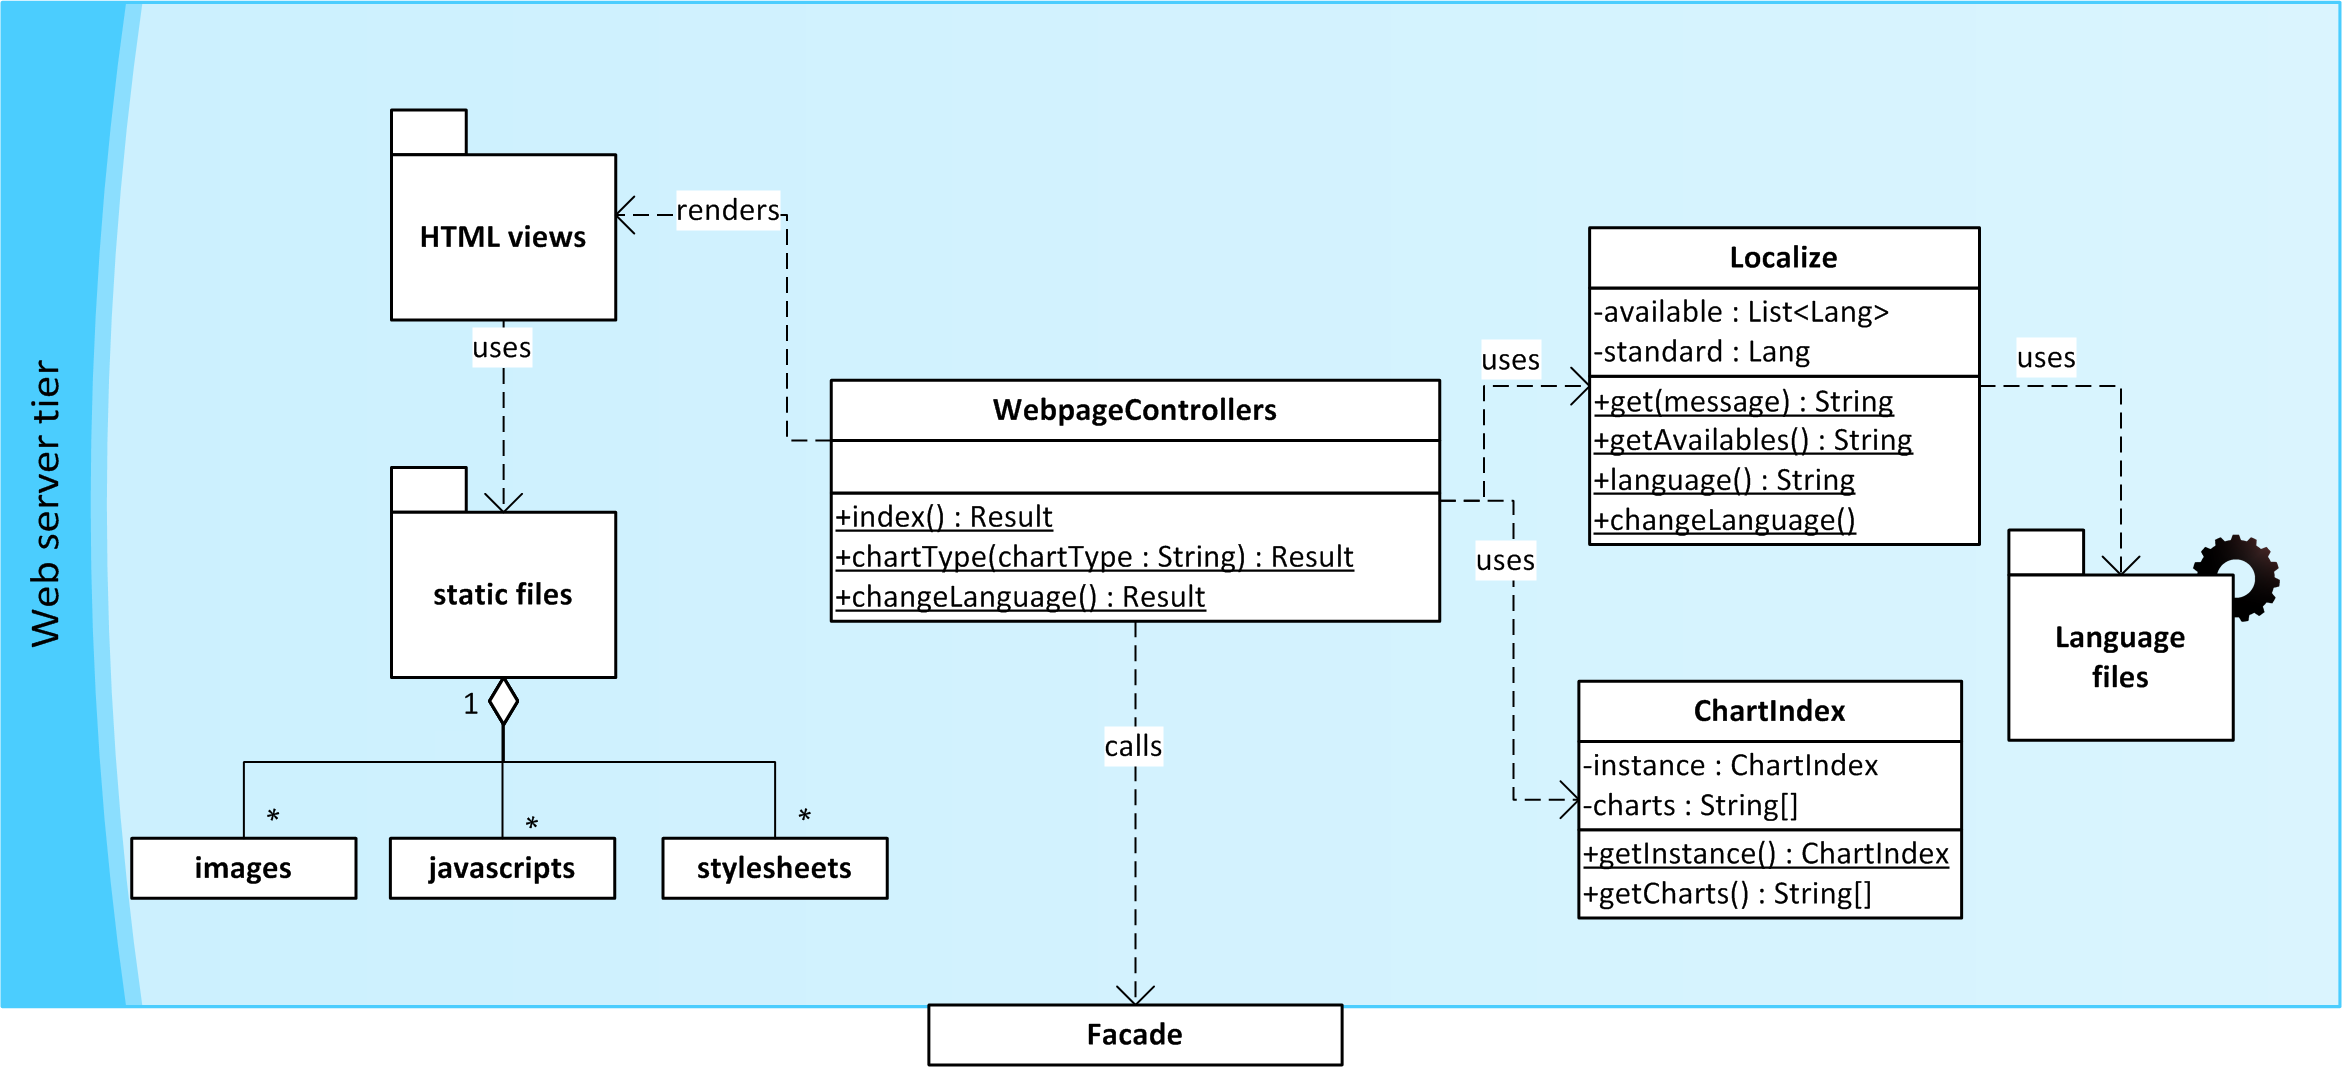
\includegraphics[width=1\linewidth]{Pictures/ServerTierDia.png}
%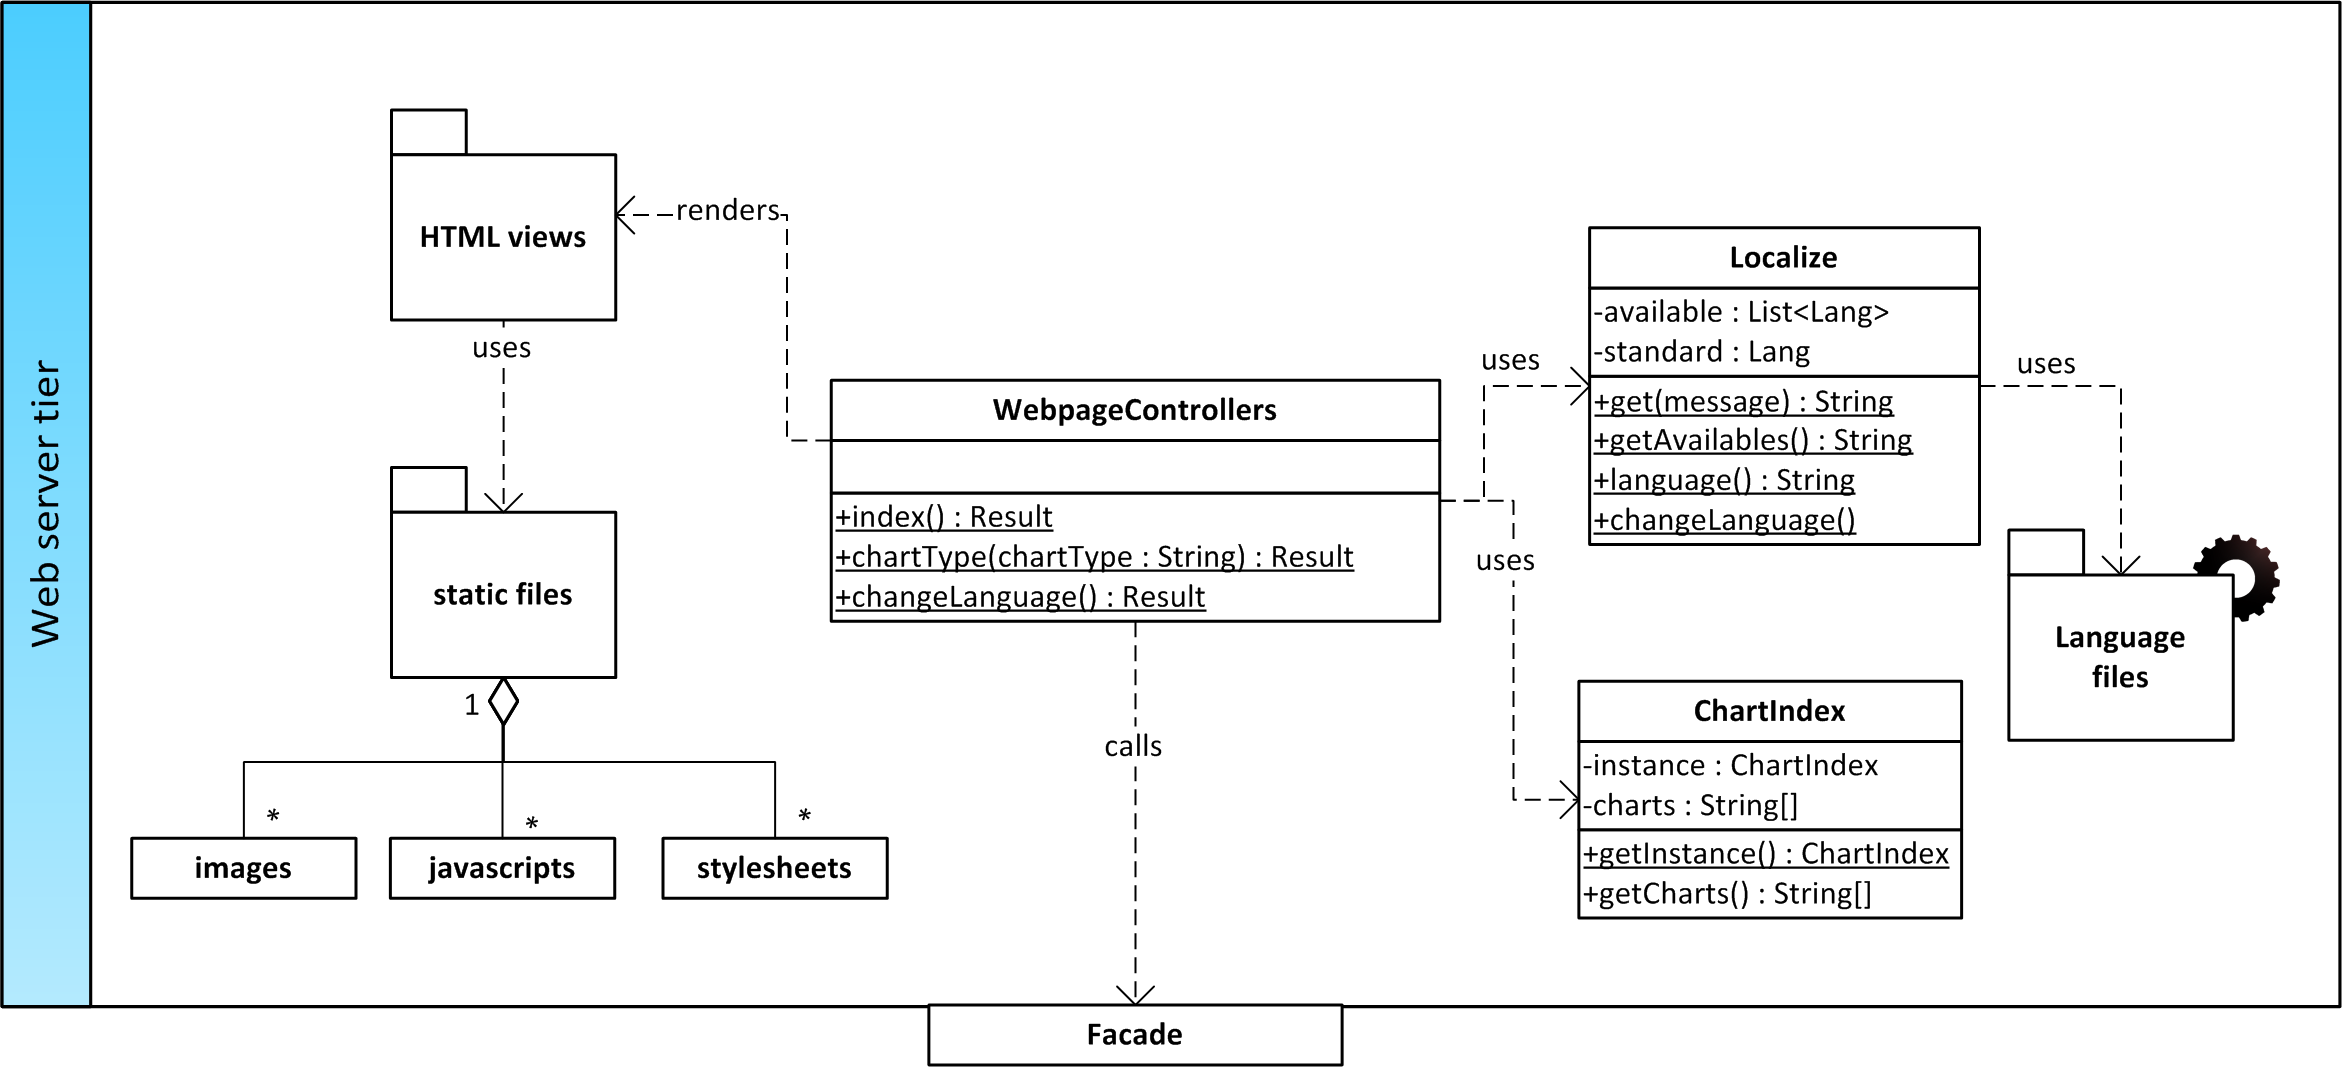
\includegraphics[width=1\linewidth]{Pictures/ServerTierDiaNormal.png} 
\end{center}   


\subsubsection*{WebpageControllers}
All valid HTTP requests are mapped to a method from WebpageControllers.
WebpageControllers either uses other helper classes to handle requests itself  
or makes calls to the facade of the application tier. 
The last step done by WebpageControllers is to create a valid HTTP response.
                                                                            

\subsubsection*{HTML views}
The HTML views contain the main template for, and all other HTML content of the webpage. %unklar
They do not have to be static, but can also dynamically integrate some content, e.g. localized strings.

\subsubsection*{Static files}
Static files contains all files of the webpage, which are not changed during runtime. 
This includes, but is not limited, to images of the webpage, javascript files and stylesheets.

\subsubsection*{Localize}
Localize is a static helper class handling all the language related things. 
It has a method to get localized Strings using the language files, 
to change the language of the webpage und methods determining all available languages, 
%dieser Satz, passt der syntaktisch? Sollte es methods sein?
so they can be integrated in the webpage once they are present.

\subsubsection*{ChartIndex}
ChartIndex implements the singleton pattern. On instantiation it scans which chart types are available 
and saves them internally. This is used by the index page to dynamically display all available chart types,
even if one is deleted or added.
%Do we have to specify how one might add them? I mean, not here, but somewhere.


\subsection{Application \& Data access tier class diagram}

TODOO sentence about this dia
\newpage
\begin{center}
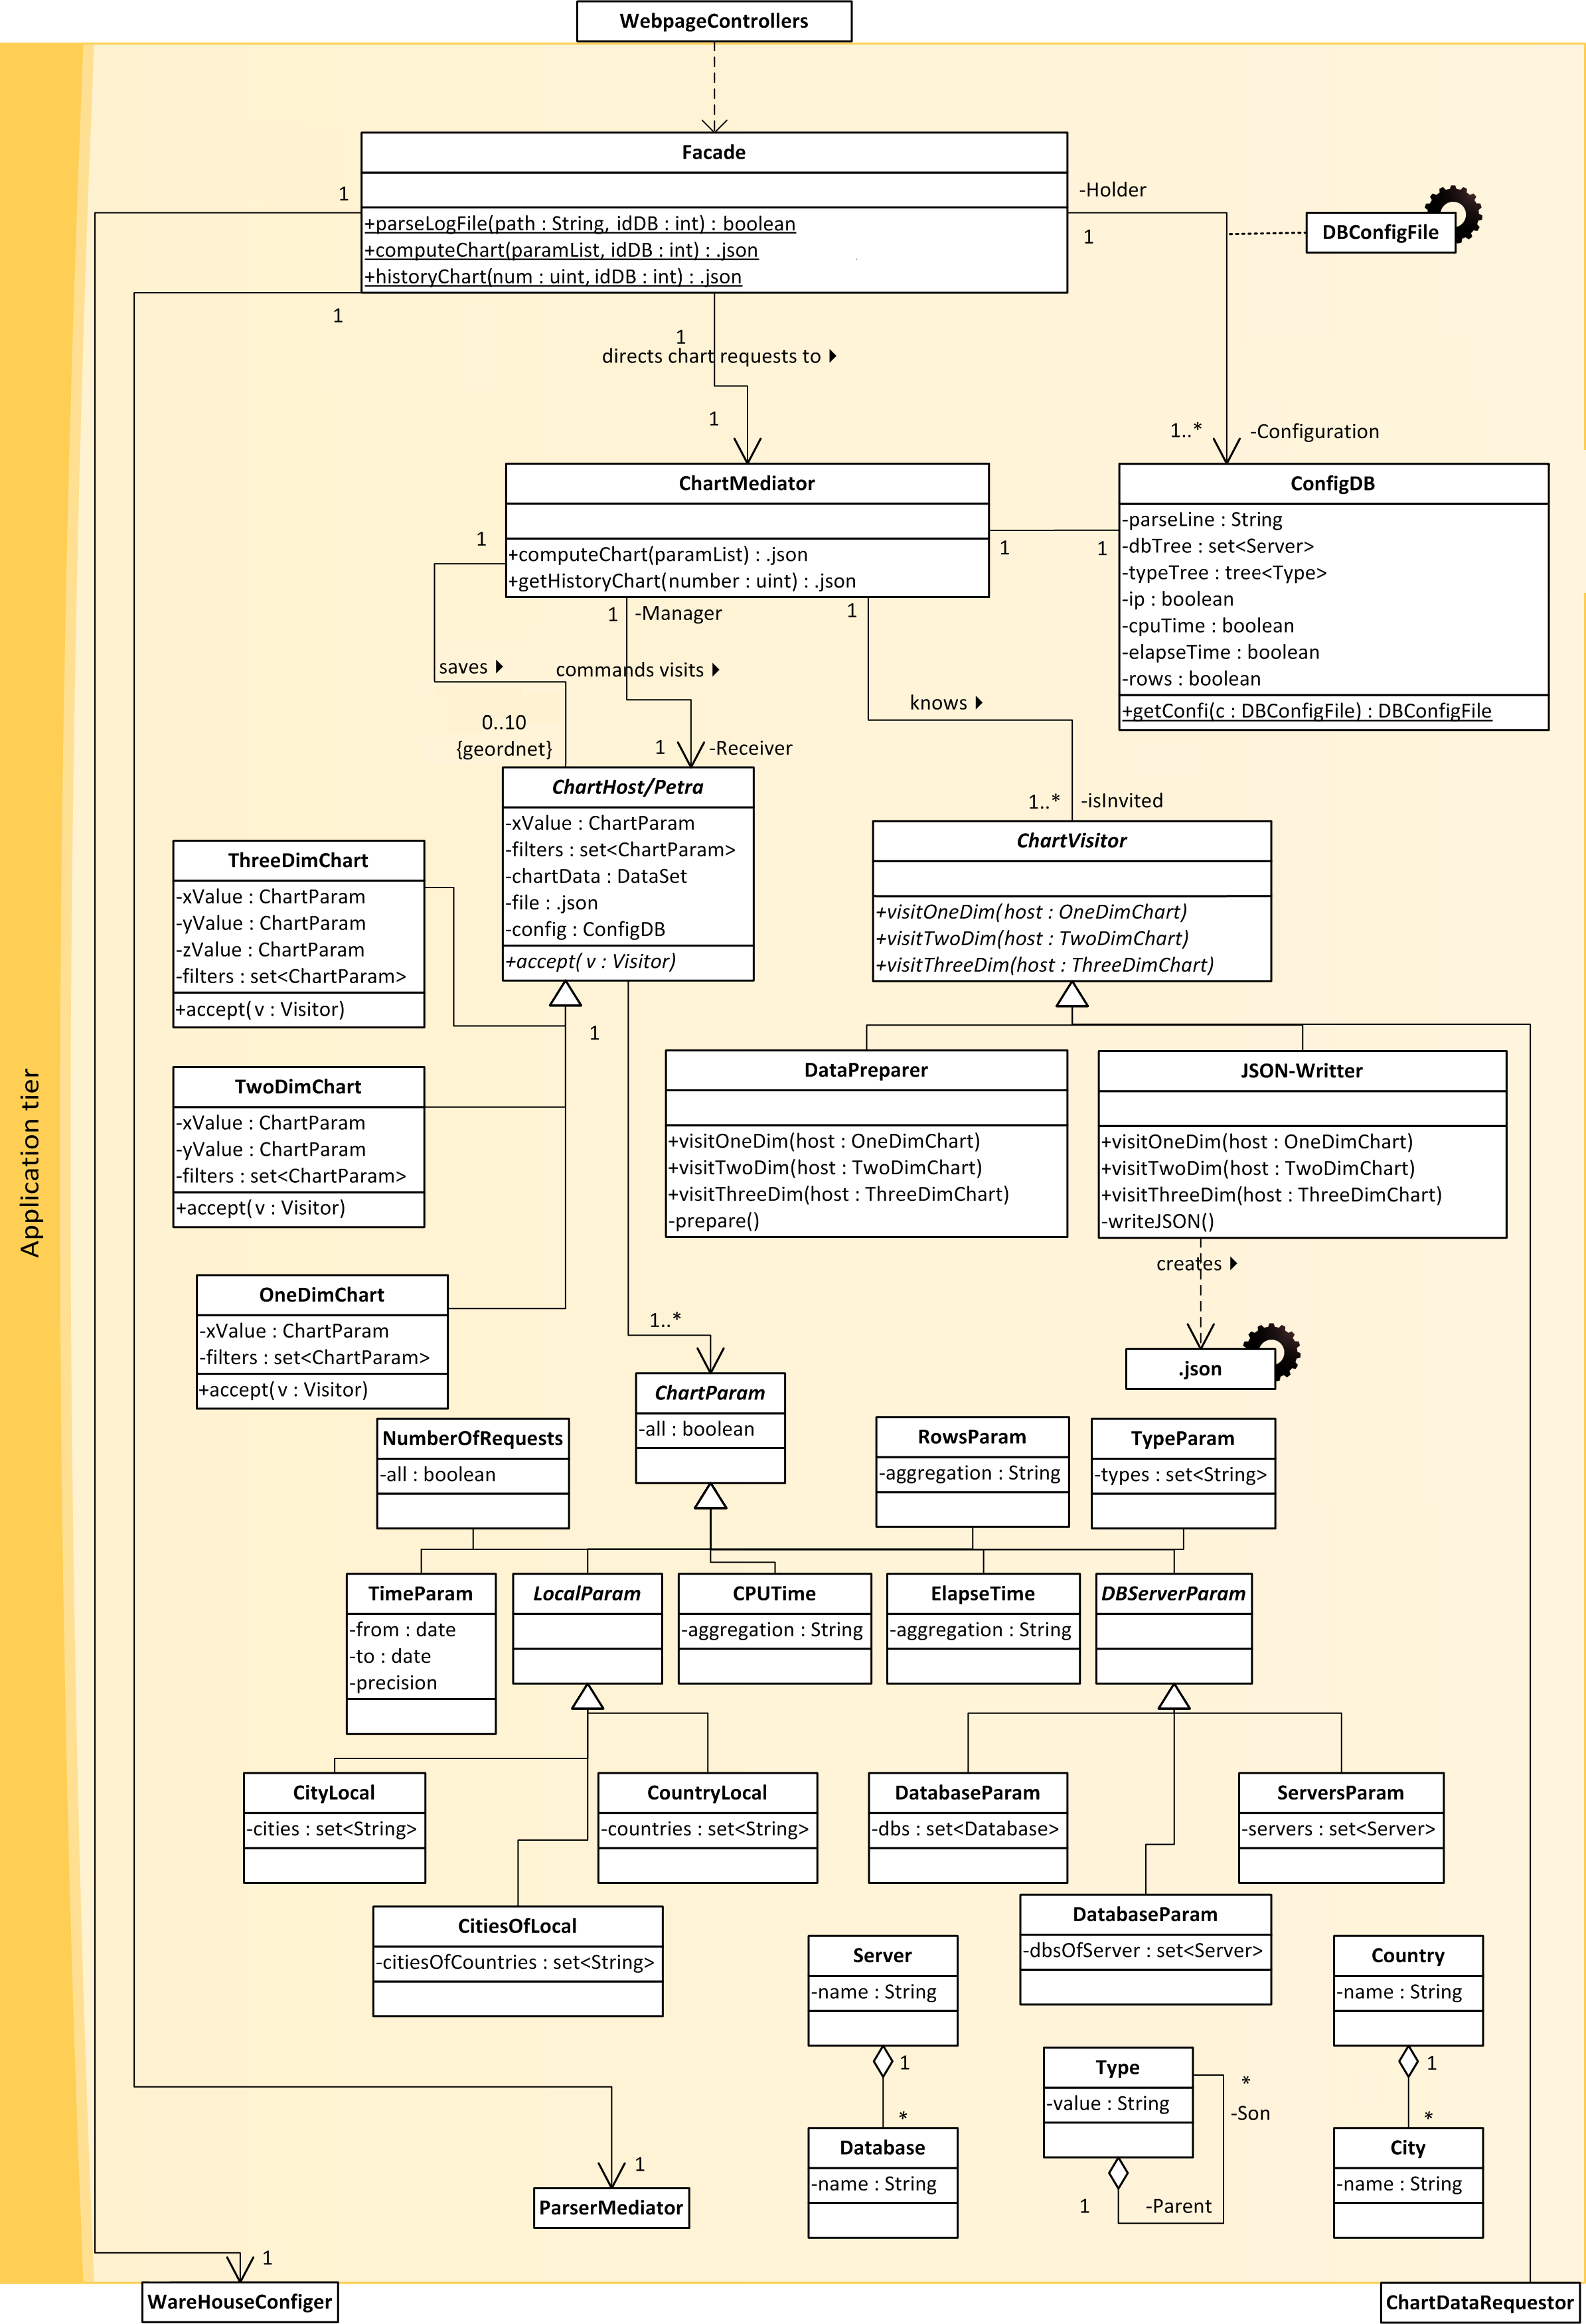
\includegraphics[width=0.9\linewidth]{Pictures/AppTierDia1.png}
%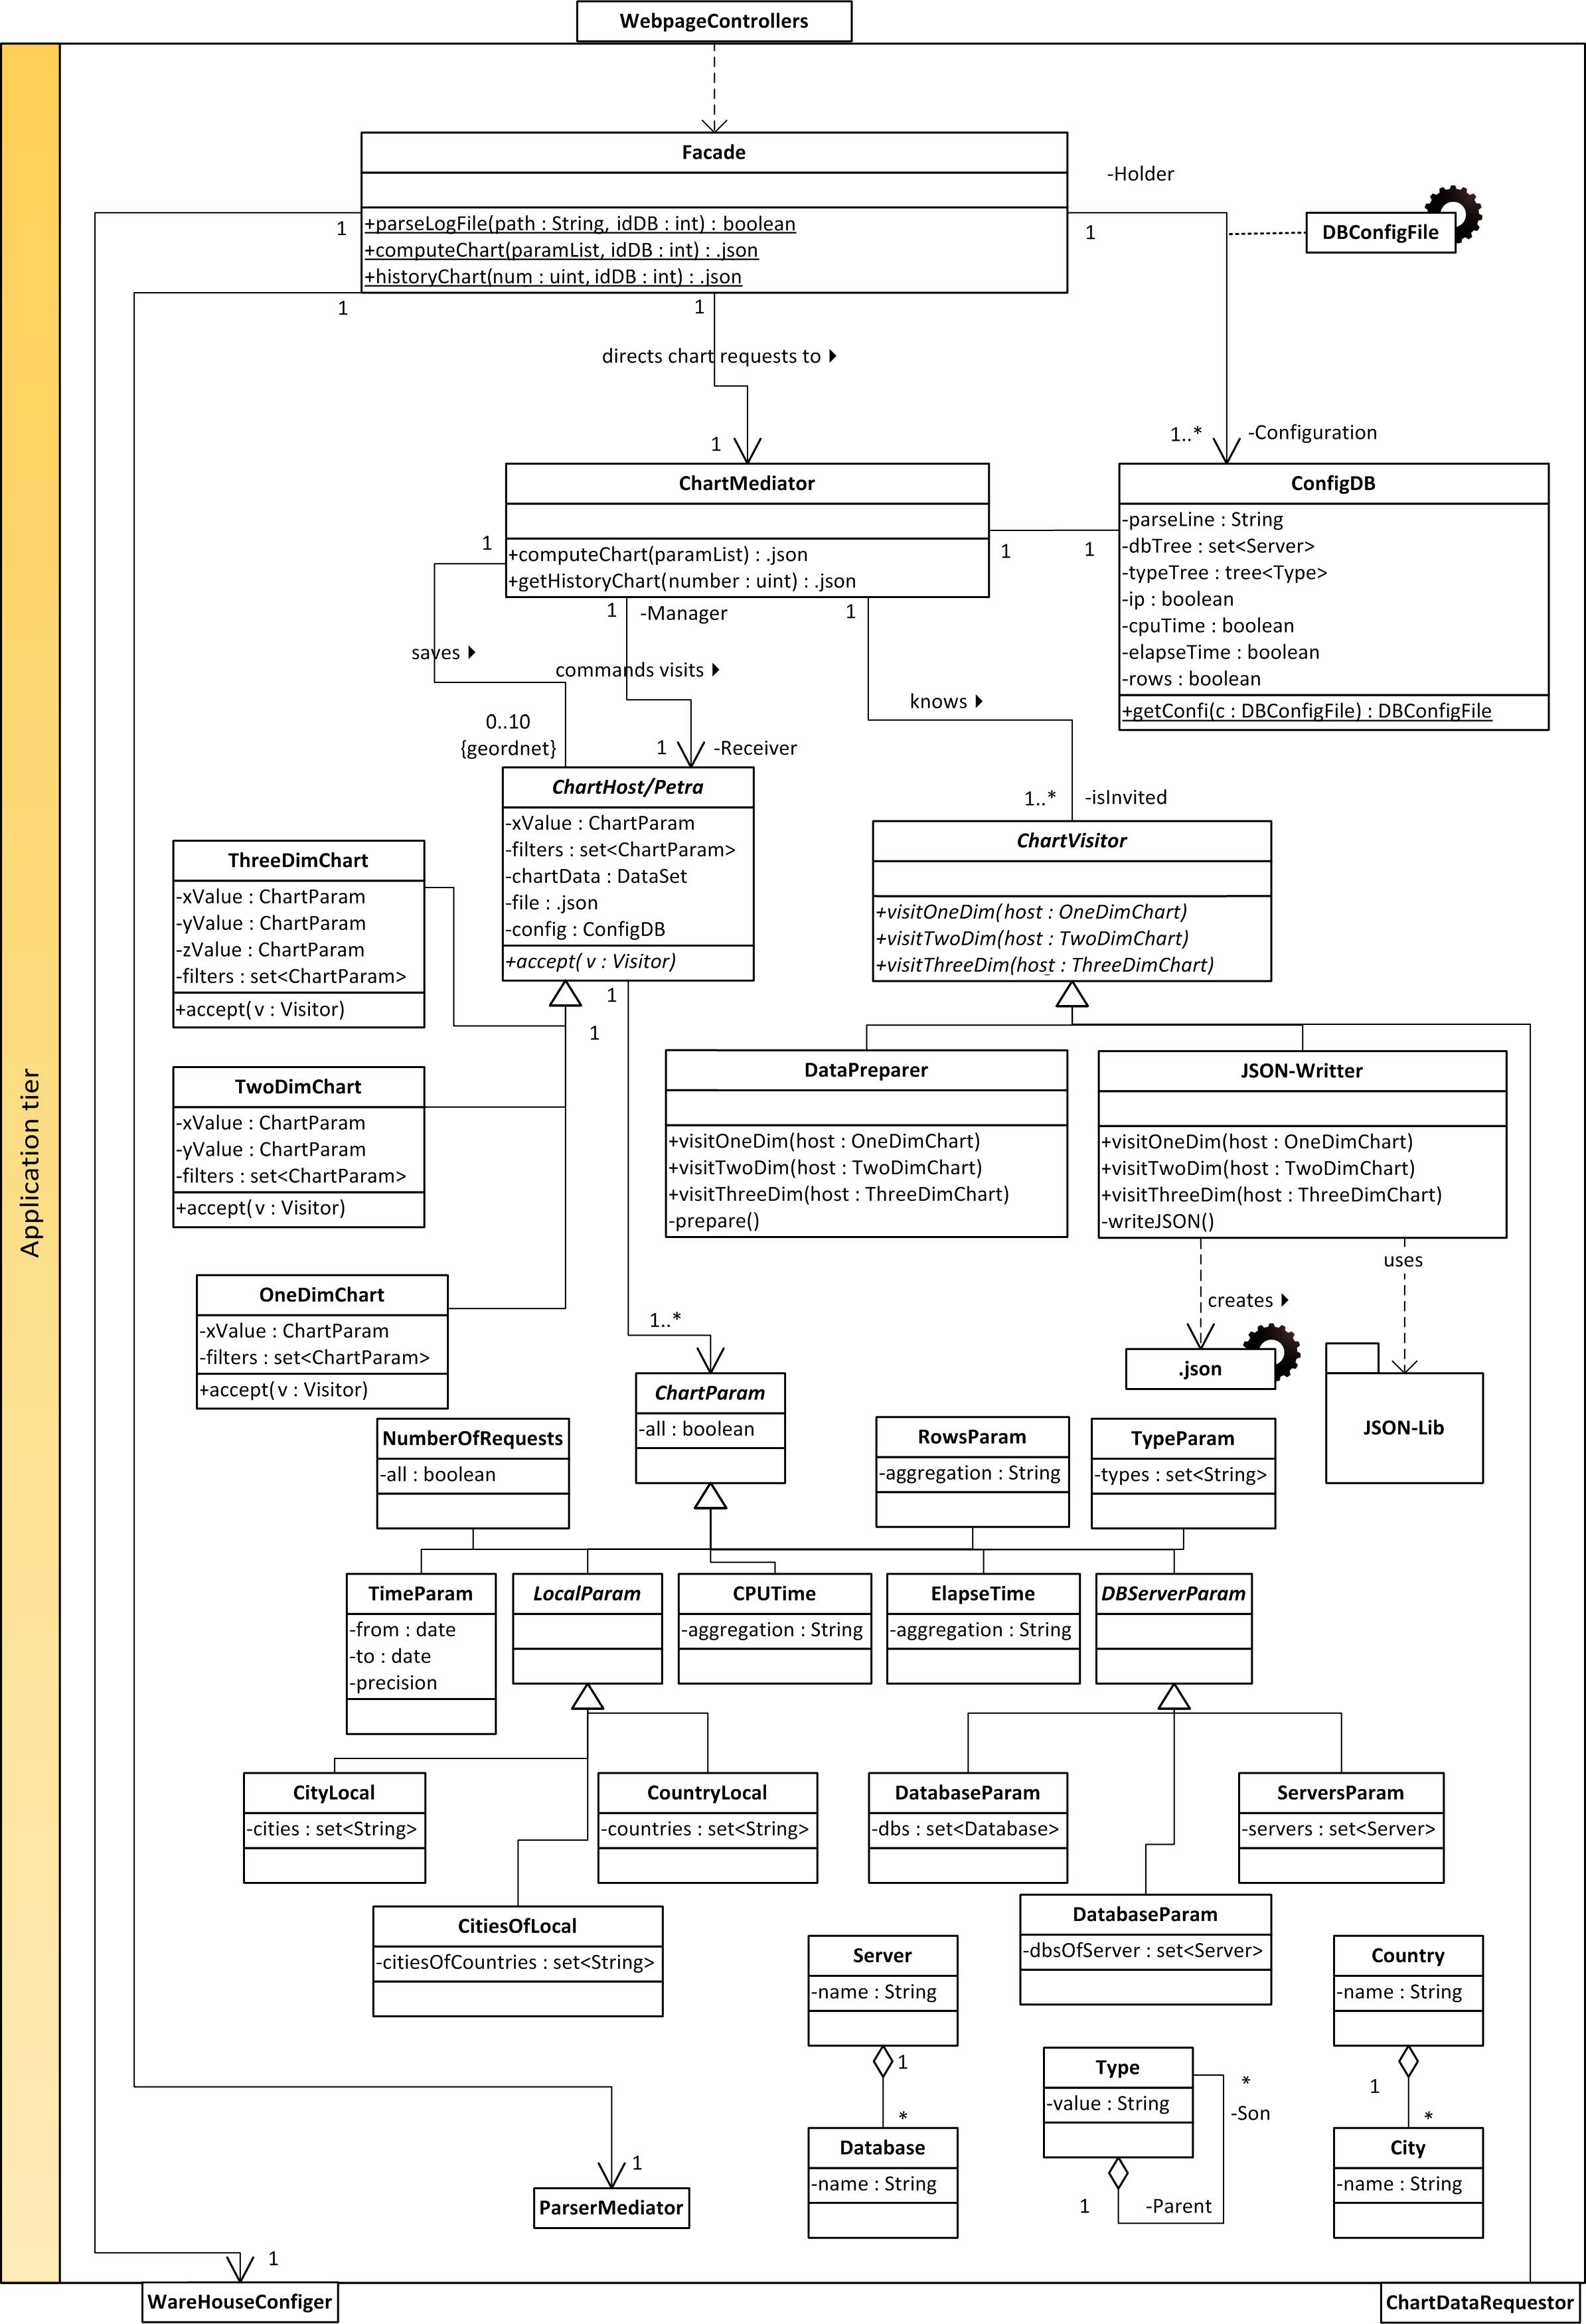
\includegraphics[width=0.9\linewidth]{Pictures/AppTierDia1Normal.png} 
\end{center}  
\begin{center}
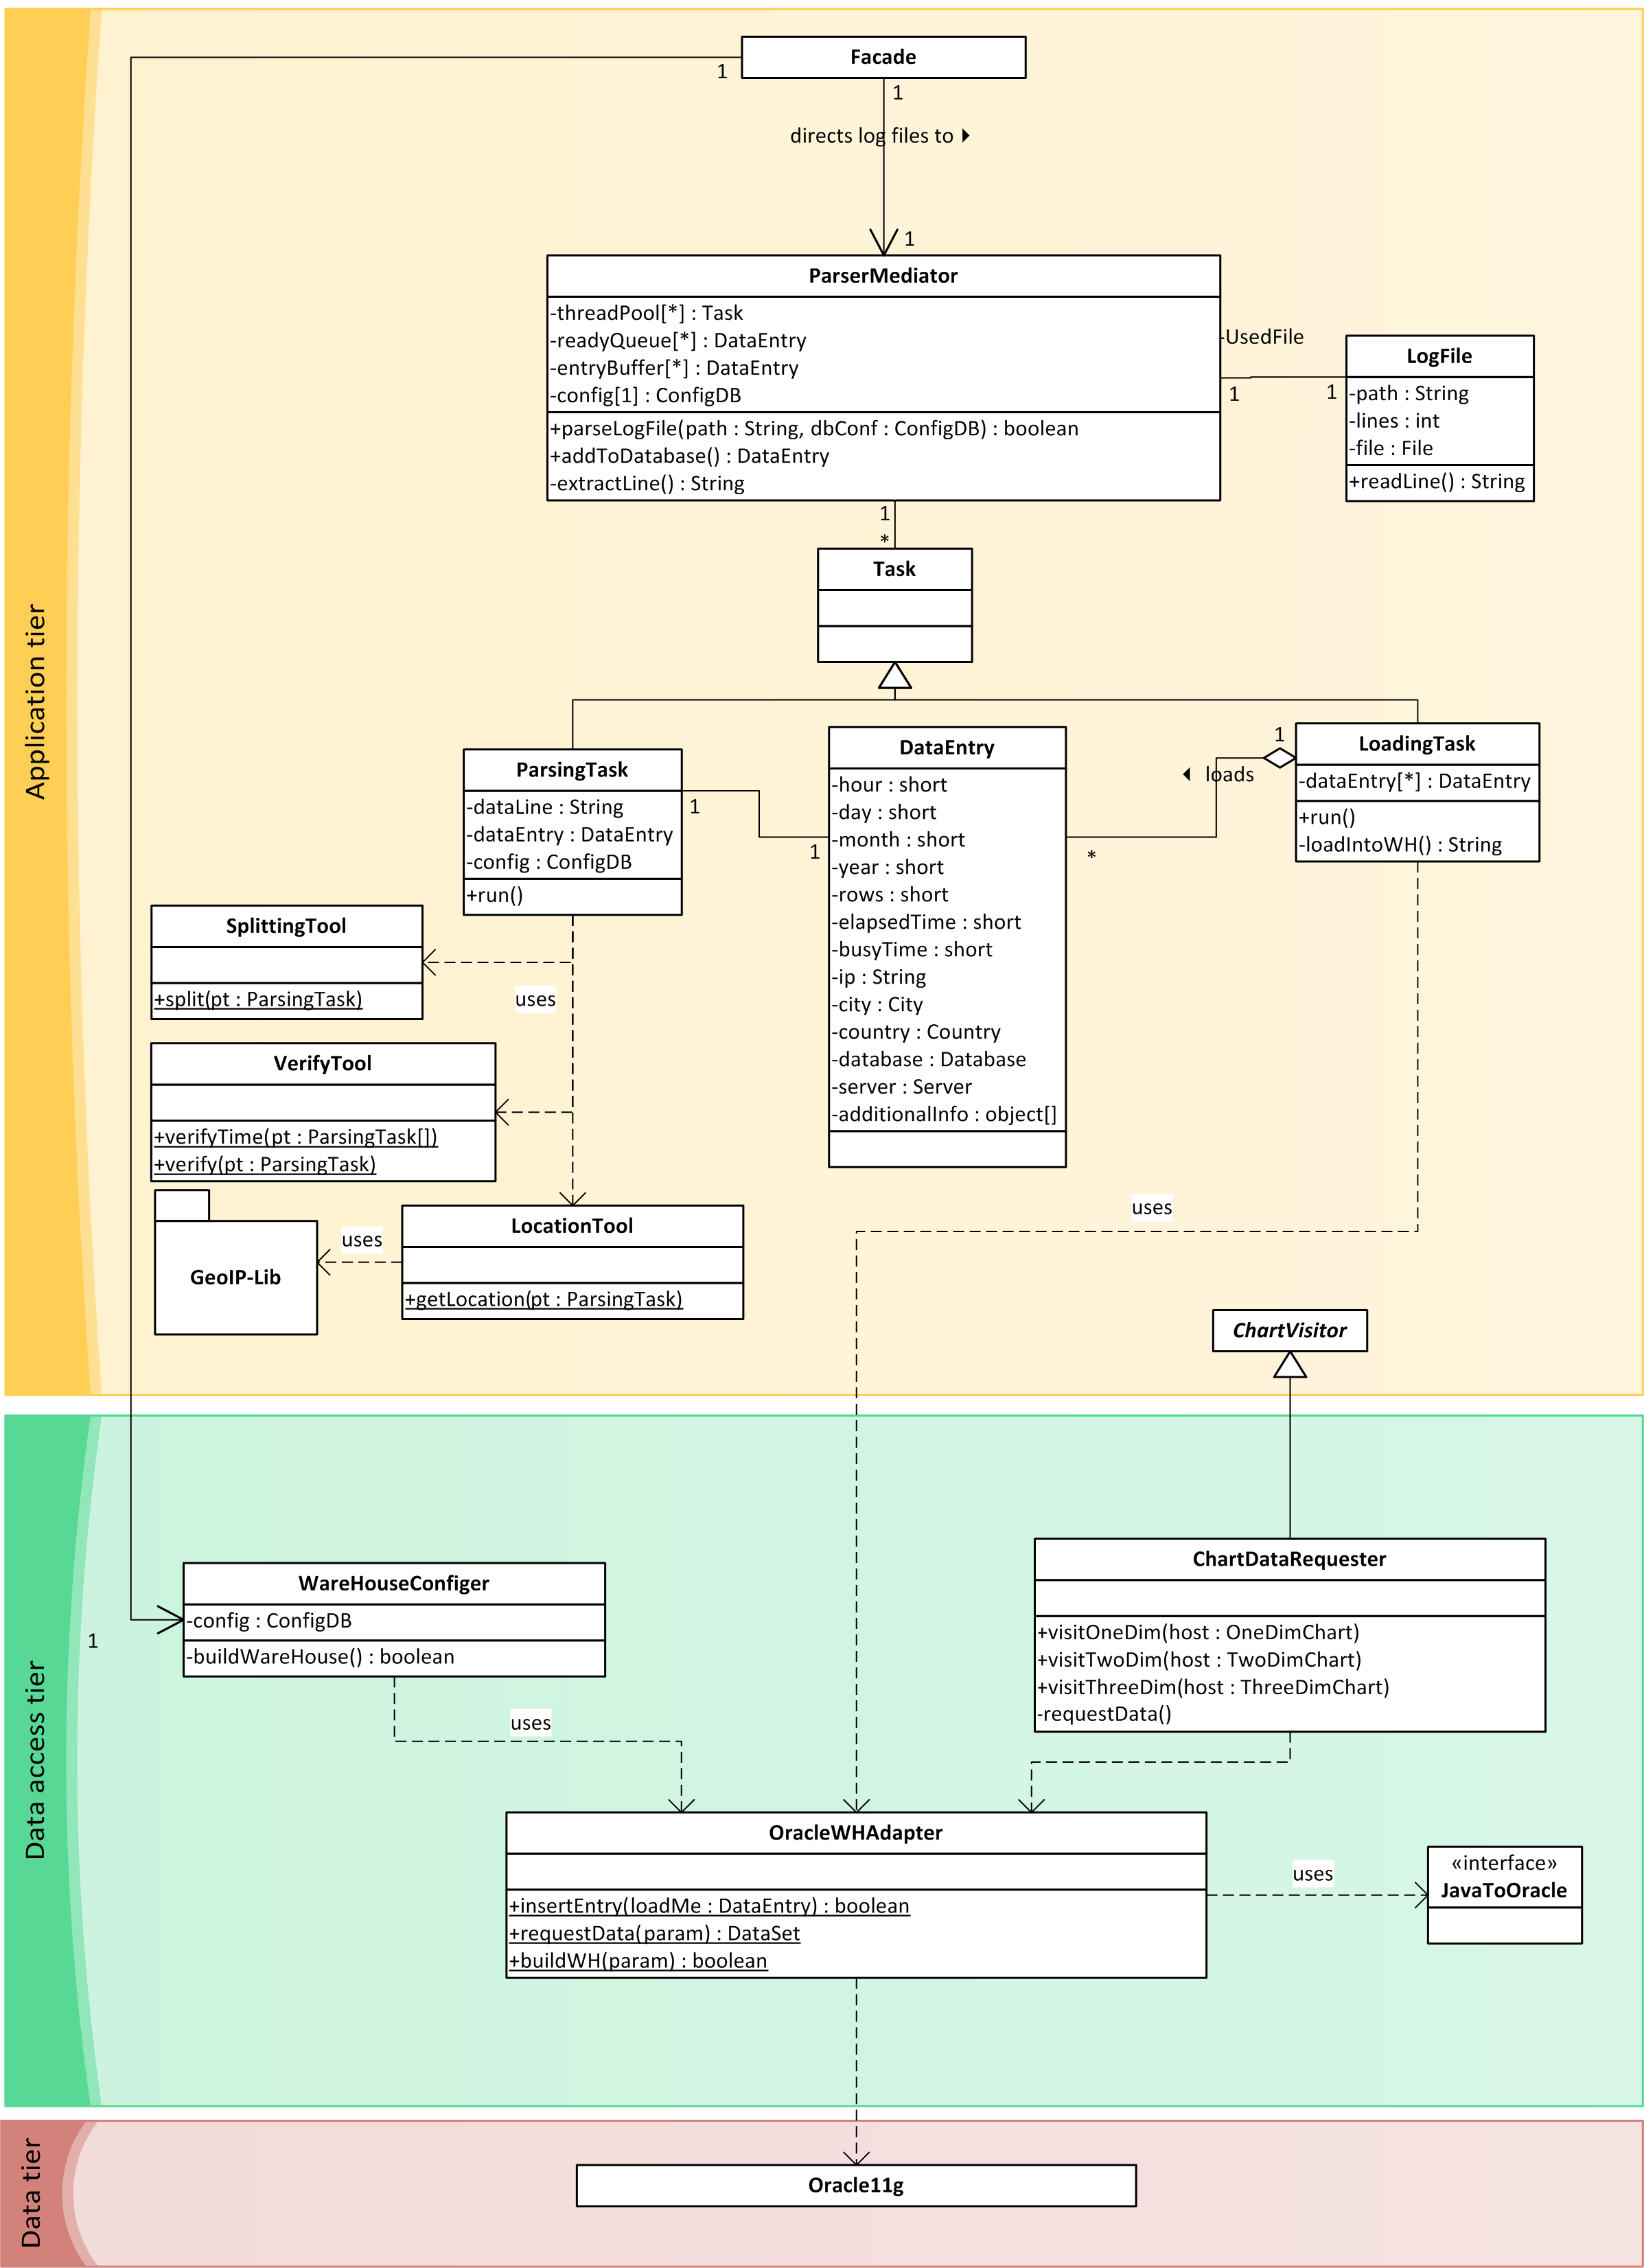
\includegraphics[width=0.9\linewidth]{Pictures/AppTierDia2.png}
%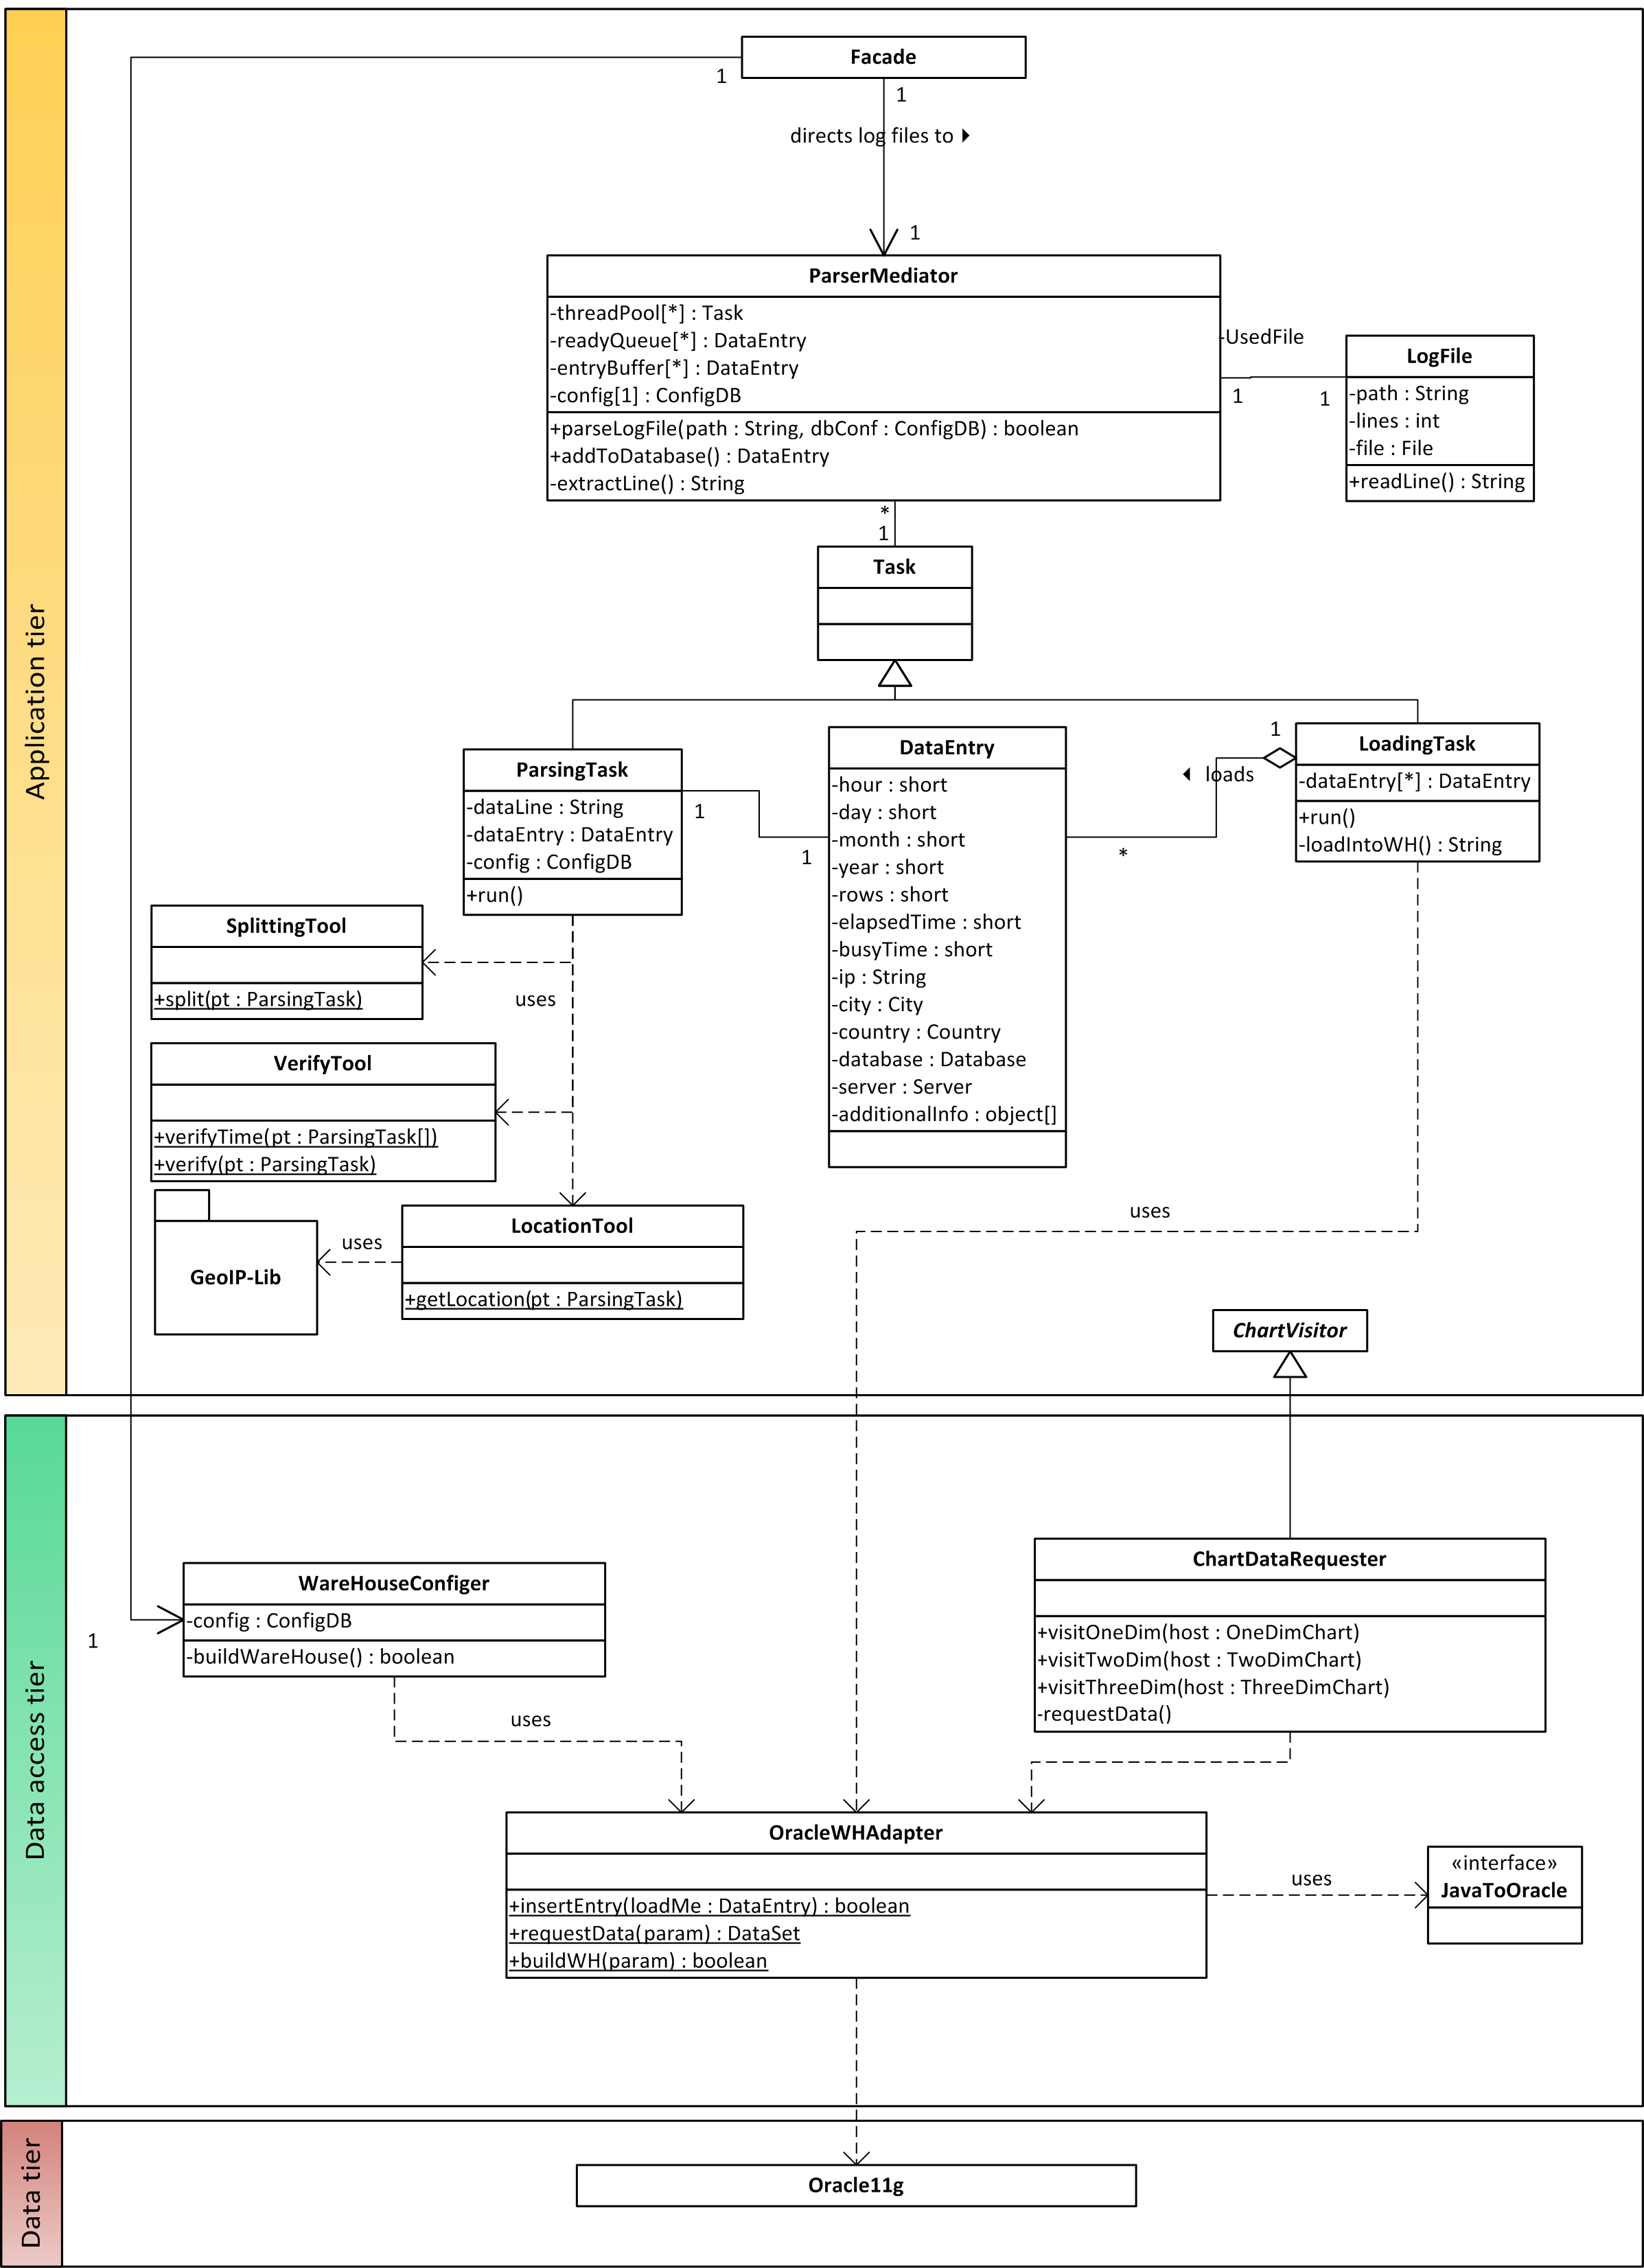
\includegraphics[width=0.9\linewidth]{Pictures/AppTierDia2Normal.png} 
\end{center}  

\subsection{Fassade + Configurations}
%picture
\subsubsection{Fassade}


\subsection{Chart request operator}
Visitor pattern blabla   
classes
%picture
\subsubsection{Fassade}

\subsection{Chart parameters}
The chart parameters describe 
\subsection{}


\subsection{Parser}

HIER LOGFILE  PARSERMEDIATOR HIN!
CAPSLOCK REGELT, UND SO!!11einself %JA, ABER DAS KANN NICHT DA BLEIBEN!!1

\subsubsection*{ParserMediator}
ParserMediator is the 'main'-Class of the Parser. It creates and administrates a threadpool, which contains several tasks, 
%contains used twice very shortly (I was momentarily confused).Also, the sentence is huge. I see no immediate replacement
contains the entryBuffer for finished DataEntries, the stringBuffer for strings, which were extracted 
from the logfile and saves which log file and configuration file is used.

\subsubsection*{LogFile}
The gateway between parser and logfile - it contains the path of the logfile and an integer 
which saves how many lines have been read from this file. It can read single lines from the logfile and return them to 
the Parser.

DATAENTRY

\subsubsection*{DataEntry}
The dataEntry which will be written in the warehouse.
It contains 
-hour, day, month, year of the request,
-rows which were read  from the logfile%from the logfile or rows accessed in the original db? %+1, it is not clear
-the elapsed and busy time on the server
-the ip from which the request came
-the type of request
-the database and server which handled the request. %I Thought I'd break this up and make a list
It may contain additional information depending on the actual logfile, as specified in the configuration file. %is this correct?

%\newline\newline doesnt work in empty lines
\subsubsection*{Java Files}
The Parser uses java.io.File and a ThreadPool from java.util.

TOOLS + PARSING TASK!

\subsubsection*{SplittingTool}
The splitting tool splits the dataLine from its parsingTask and enters the splitted parts into the dataEntry.

\subsubsection*{VerifyTool}
The VerifyTool checks if the dataEntry is correct - if it has a mistake (e.g. Month = 13 or Elapsed Time = -1), it will 
be deleted and the VerifyTool sends an detailed error, which can be displayed elsewhere.

\subsubsection*{LocationTool}
The LocationTool takes the IP from the dataEntry and uses GeoIP-libraries[geo] to determine the city and country of the request.
Those will be added to the dataEntry.

\subsubsection*{ParsingTask}
A ParsingTask is one of the tasks which are created from Parser. It gets a line from the logfile and uses, SplittingTool, VerifyTool
and LocationTool to create a dataEntry which contains the same information. 

LOADING TASK! %ARE WE ALLOWED TO BE EXCITED?


\subsubsection*{LoadingTask}
A loading task is another possible task for the threadPool. It takes a finished dataEntry from the buffer and sends it to the warehouse.

\subsubsection*{WareHouseGonfiger}

This Config sends the order to OracleWHAdapter to build the Data Warehouse.

\subsubsection*{ChartDataRequester}

A ChartDataRequester is a request which get its information from ChartVistor
and sends the data in request form to OracleWHAdapter. %I don't understand this
The response of this class is to build data for the requester.

\subsubsection*{OracleWHAdapter}

After accessing the Database and geting the DataEntry from LoadingTask then will build %who?
the data warehouse in OLAP - Cube form. With help from Oracle %Sounds like a group of superheroes saving the world!
and Java library, which make it easy to access the database and build the warehouse. %I though the warehouse was built before
 
\subsubsection*{JavaToOracle}

Is a Library interface, wich makes a connection with a database.

\subsubsection*{Oracle}

A database language. %is it?

geo
 link to the maxmind geoip library in the library section
